\chapter{Combinatorics}

\index{combinatorics}

\key{Combinatorics} studies methods for counting
combinations of objects.
Usually, the goal is to find a way to
count the combinations efficiently
without generating each combination separately.

As an example, consider the problem
of counting the number of ways to
represent an integer $n$ as a sum of positive integers.
For example, there are 8 representations
for $4$:
\begin{multicols}{2}
\begin{itemize}
\item $1+1+1+1$
\item $1+1+2$
\item $1+2+1$
\item $2+1+1$
\item $2+2$
\item $3+1$
\item $1+3$
\item $4$
\end{itemize}
\end{multicols}

A combinatorial problem can often be solved
using a recursive function.
In this problem, we can define a function $f(n)$
that gives the number of representations for $n$.
For example, $f(4)=8$ according to the above example.
The values of the function
can be recursively calculated as follows:
\begin{equation*}
    f(n) = \begin{cases}
               1               & n = 0\\
               f(0)+f(1)+\cdots+f(n-1) & n > 0\\
           \end{cases}
\end{equation*}
The base case is $f(0)=1$,
because the empty sum represents the number 0.
Then, if $n>0$, we consider all ways to
choose the first number of the sum.
If the first number is $k$,
there are $f(n-k)$ representations
for the remaining part of the sum.
Thus, we calculate the sum of all values
of the form $f(n-k)$ where $k<n$.

The first values for the function are:
\[
\begin{array}{lcl}
f(0) & = & 1 \\
f(1) & = & 1 \\
f(2) & = & 2 \\
f(3) & = & 4 \\
f(4) & = & 8 \\
\end{array}
\]

Sometimes, a recursive formula can be replaced
with a closed-form formula.
In this problem,
\[
f(n)=2^{n-1},
\]
which is based on the fact that there are $n-1$
possible positions for +-signs in the sum
and we can choose any subset of them.

\section{Binomial coefficients}

\index{binomial coefficient}

The \key{binomial coefficient} ${n \choose k}$
equals the number of ways we can choose a subset
of $k$ elements from a set of $n$ elements.
For example, ${5 \choose 3}=10$,
because the set $\{1,2,3,4,5\}$
has 10 subsets of 3 elements:
\[ \{1,2,3\}, \{1,2,4\}, \{1,2,5\}, \{1,3,4\}, \{1,3,5\}, 
\{1,4,5\}, \{2,3,4\}, \{2,3,5\}, \{2,4,5\}, \{3,4,5\} \]

\subsubsection{Formula 1}

Binomial coefficients can be
recursively calculated as follows:

\[
{n \choose k}  =  {n-1 \choose k-1} + {n-1 \choose k}
\]

The idea is to fix an element $x$ in the set.
If $x$ is included in the subset,
we have to choose $k-1$
elements from $n-1$ elements,
and if $x$ is not included in the subset,
we have to choose $k$ elements from $n-1$ elements.

The base cases for the recursion are
\[
{n \choose 0}  =  {n \choose n} = 1,
\]
because there is always exactly
one way to construct an empty subset
and a subset that contains all the elements.

\subsubsection{Formula 2}

Another way to calculate binomial coefficients is as follows:
\[
{n \choose k}  =  \frac{n!}{k!(n-k)!}.
\]

There are $n!$ permutations of $n$ elements.
We go through all permutations and always
include the first $k$ elements of the permutation
in the subset.
Since the order of the elements in the subset
and outside the subset does not matter,
the result is divided by $k!$ and $(n-k)!$

\subsubsection{Properties}

For binomial coefficients,
\[
{n \choose k}  =  {n \choose n-k},
\]
because we actually divide a set of $n$ elements into
two subsets: the first contains $k$ elements
and the second contains $n-k$ elements.

The sum of binomial coefficients is
\[
{n \choose 0}+{n \choose 1}+{n \choose 2}+\ldots+{n \choose n}=2^n.
\]

The reason for the name ''binomial coefficient''
can be seen when the binomial $(a+b)$ is raised to
the $n$th power:

\[ (a+b)^n =
{n \choose 0} a^n b^0 + 
{n \choose 1} a^{n-1} b^1 +
\ldots + 
{n \choose n-1} a^1 b^{n-1} +
{n \choose n} a^0 b^n. \]

\index{Pascal's triangle}

Binomial coefficients also appear in
\key{Pascal's triangle}
where each value equals the sum of two
above values:
\begin{center}
\begin{tikzpicture}{0.9}
\node at (0,0) {1};
\node at (-0.5,-0.5) {1};
\node at (0.5,-0.5) {1};
\node at (-1,-1) {1};
\node at (0,-1) {2};
\node at (1,-1) {1};
\node at (-1.5,-1.5) {1};
\node at (-0.5,-1.5) {3};
\node at (0.5,-1.5) {3};
\node at (1.5,-1.5) {1};
\node at (-2,-2) {1};
\node at (-1,-2) {4};
\node at (0,-2) {6};
\node at (1,-2) {4};
\node at (2,-2) {1};
\node at (-2,-2.5) {$\ldots$};
\node at (-1,-2.5) {$\ldots$};
\node at (0,-2.5) {$\ldots$};
\node at (1,-2.5) {$\ldots$};
\node at (2,-2.5) {$\ldots$};
\end{tikzpicture}
\end{center}

\subsubsection{Boxes and balls}

''Boxes and balls'' is a useful model,
where we count the ways to
place $k$ balls in $n$ boxes.
Let us consider three scenarios:

\textit{Scenario 1}: Each box can contain
at most one ball.
For example, when $n=5$ and $k=2$,
there are 10 solutions:

\begin{center}
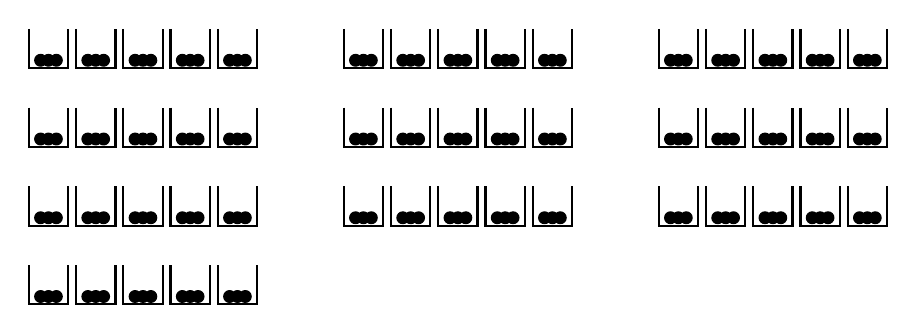
\begin{tikzpicture}[scale=0.5]
\newcommand\lax[3]{
\path[draw,thick,-] (#1-0.5,#2+0.5) -- (#1-0.5,#2-0.5) --
                    (#1+0.5,#2-0.5) -- (#1+0.5,#2+0.5);
\ifthenelse{\equal{#3}{1}}{\draw[fill=black] (#1,#2-0.3) circle (0.15);}{}
\ifthenelse{\equal{#3}{2}}{\draw[fill=black] (#1-0.2,#2-0.3) circle (0.15);}{}
\ifthenelse{\equal{#3}{2}}{\draw[fill=black] (#1+0.2,#2-0.3) circle (0.15);}{}
}
\newcommand\laa[7]{
    \lax{#1}{#2}{#3}
    \lax{#1+1.2}{#2}{#4}
    \lax{#1+2.4}{#2}{#5}
    \lax{#1+3.6}{#2}{#6}
    \lax{#1+4.8}{#2}{#7}
}

\laa{0}{0}{1}{1}{0}{0}{0}
\laa{0}{-2}{1}{0}{1}{0}{0}
\laa{0}{-4}{1}{0}{0}{1}{0}
\laa{0}{-6}{1}{0}{0}{0}{1}
\laa{8}{0}{0}{1}{1}{0}{0}
\laa{8}{-2}{0}{1}{0}{1}{0}
\laa{8}{-4}{0}{1}{0}{0}{1}
\laa{16}{0}{0}{0}{1}{1}{0}
\laa{16}{-2}{0}{0}{1}{0}{1}
\laa{16}{-4}{0}{0}{0}{1}{1}

\end{tikzpicture}
\end{center}

In this scenario, the answer is directly the
binomial coefficient ${n \choose k}$.

\textit{Scenario 2}: A box can contain multiple balls.
For example, when $n=5$ and $k=2$,
there are 15 solutions:

\begin{center}
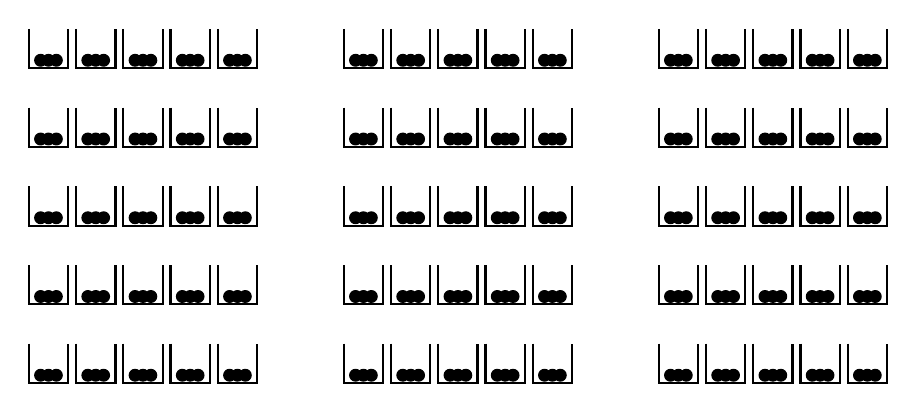
\begin{tikzpicture}[scale=0.5]
\newcommand\lax[3]{
\path[draw,thick,-] (#1-0.5,#2+0.5) -- (#1-0.5,#2-0.5) --
                    (#1+0.5,#2-0.5) -- (#1+0.5,#2+0.5);
\ifthenelse{\equal{#3}{1}}{\draw[fill=black] (#1,#2-0.3) circle (0.15);}{}
\ifthenelse{\equal{#3}{2}}{\draw[fill=black] (#1-0.2,#2-0.3) circle (0.15);}{}
\ifthenelse{\equal{#3}{2}}{\draw[fill=black] (#1+0.2,#2-0.3) circle (0.15);}{}
}
\newcommand\laa[7]{
    \lax{#1}{#2}{#3}
    \lax{#1+1.2}{#2}{#4}
    \lax{#1+2.4}{#2}{#5}
    \lax{#1+3.6}{#2}{#6}
    \lax{#1+4.8}{#2}{#7}
}

\laa{0}{0}{2}{0}{0}{0}{0}
\laa{0}{-2}{1}{1}{0}{0}{0}
\laa{0}{-4}{1}{0}{1}{0}{0}
\laa{0}{-6}{1}{0}{0}{1}{0}
\laa{0}{-8}{1}{0}{0}{0}{1}
\laa{8}{0}{0}{2}{0}{0}{0}
\laa{8}{-2}{0}{1}{1}{0}{0}
\laa{8}{-4}{0}{1}{0}{1}{0}
\laa{8}{-6}{0}{1}{0}{0}{1}
\laa{8}{-8}{0}{0}{2}{0}{0}
\laa{16}{0}{0}{0}{1}{1}{0}
\laa{16}{-2}{0}{0}{1}{0}{1}
\laa{16}{-4}{0}{0}{0}{2}{0}
\laa{16}{-6}{0}{0}{0}{1}{1}
\laa{16}{-8}{0}{0}{0}{0}{2}

\end{tikzpicture}
\end{center}

The process of placing the balls in the boxes
can be represented as a string
that consists of symbols
''o'' and ''$\rightarrow$''.
Initially, assume that we are standing at the leftmost box.
The symbol ''o'' means that we place a ball
in the current box, and the symbol
''$\rightarrow$'' means that we move to
the next box to the right.

Using this notation, each solution is a string
that contains $k$ times the symbol ''o'' and
$n-1$ times the symbol ''$\rightarrow$''.
For example, the upper-right solution
in the above picture corresponds to the string
''$\rightarrow$ $\rightarrow$ o $\rightarrow$ o $\rightarrow$''.
Thus, the number of solutions is
${k+n-1 \choose k}$.

\textit{Scenario 3}: Each box may contain at most one ball,
and in addition, no two adjacent boxes may both contain a ball.
For example, when $n=5$ and $k=2$,
there are 6 solutions:


\begin{center}
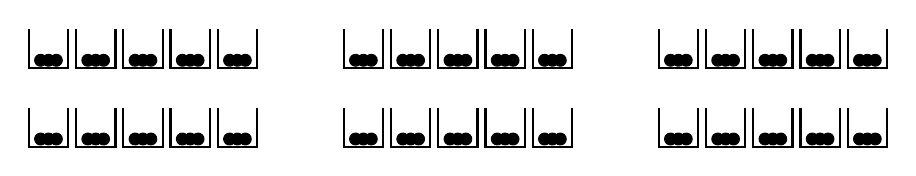
\begin{tikzpicture}[scale=0.5]
\newcommand\lax[3]{
\path[draw,thick,-] (#1-0.5,#2+0.5) -- (#1-0.5,#2-0.5) --
                    (#1+0.5,#2-0.5) -- (#1+0.5,#2+0.5);
\ifthenelse{\equal{#3}{1}}{\draw[fill=black] (#1,#2-0.3) circle (0.15);}{}
\ifthenelse{\equal{#3}{2}}{\draw[fill=black] (#1-0.2,#2-0.3) circle (0.15);}{}
\ifthenelse{\equal{#3}{2}}{\draw[fill=black] (#1+0.2,#2-0.3) circle (0.15);}{}
}
\newcommand\laa[7]{
    \lax{#1}{#2}{#3}
    \lax{#1+1.2}{#2}{#4}
    \lax{#1+2.4}{#2}{#5}
    \lax{#1+3.6}{#2}{#6}
    \lax{#1+4.8}{#2}{#7}
}

\laa{0}{0}{1}{0}{1}{0}{0}
\laa{0}{-2}{1}{0}{0}{1}{0}
\laa{8}{0}{1}{0}{0}{0}{1}
\laa{8}{-2}{0}{1}{0}{1}{0}
\laa{16}{0}{0}{1}{0}{0}{1}
\laa{16}{-2}{0}{0}{1}{0}{1}
\end{tikzpicture}
\end{center}

In this scenario, we can assume that
$k$ balls are initially placed in boxes
and there is an empty box between each
two adjacent boxes.
The remaining task is to choose the
positions for the remaining empty boxes.
There are $n-2k+1$ such boxes and
$k+1$ positions for them.
Thus, using the formula of scenario 2,
the number of solutions is
${n-k+1 \choose n-2k+1}$.

\subsubsection{Multinomial coefficients}

\index{multinomial coefficient}

The \key{multinomial coefficient}
\[ {n \choose k_1,k_2,\ldots,k_m} = \frac{n!}{k_1! k_2! \cdots k_m!}, \]
equals the number of ways
we can divide $n$ elements into subsets
of sizes $k_1,k_2,\ldots,k_m$,
where $k_1+k_2+\cdots+k_m=n$.
Multinomial coefficients can be seen as a
generalization of binomial cofficients;
if $m=2$, the above formula
corresponds to the binomial coefficient formula.

\section{Catalan numbers}

\index{Catalan number}

The \key{Catalan number}
%\footnote{E. C. Catalan (1814--1894) was a Belgian mathematician.}
$C_n$ equals the
number of valid
parenthesis expressions that consist of
$n$ left parentheses and $n$ right parentheses.

For example, $C_3=5$, because
we can construct the following parenthesis
expressions using three
left and right parentheses:

\begin{itemize}[noitemsep]
\item \texttt{()()()}
\item \texttt{(())()}
\item \texttt{()(())}
\item \texttt{((()))}
\item \texttt{(()())}
\end{itemize}

\subsubsection{Parenthesis expressions}

\index{parenthesis expression}

What is exactly a \emph{valid parenthesis expression}?
The following rules precisely define all
valid parenthesis expressions:

\begin{itemize}
\item An empty parenthesis expression is valid.
\item If an expression $A$ is valid,
then also the expression
\texttt{(}$A$\texttt{)} is valid.
\item If expressions $A$ and $B$ are valid,
then also the expression $AB$ is valid.
\end{itemize}

Another way to characterize valid 
parenthesis expressions is that if
we choose any prefix of such an expression,
it has to contain at least as many left
parentheses as right parentheses.
In addition, the complete expression has to
contain an equal number of left and right
parentheses.

\subsubsection{Formula 1}

Catalan numbers can be calculated using the formula
\[ C_n = \sum_{i=0}^{n-1} C_{i} C_{n-i-1}.\]

The sum goes through the ways to divide the
expression into two parts
such that both parts are valid
expressions and the first part is as short as possible
but not empty.
For any $i$, the first part contains $i+1$ pairs
of parentheses and the number of expressions
is the product of the following values:

\begin{itemize}
\item $C_{i}$: the number of ways to construct an expression
using the parentheses of the first part,
not counting the outermost parentheses
\item $C_{n-i-1}$: the number of ways to construct an
expression using the parentheses of the second part
\end{itemize}

The base case is $C_0=1$,
because we can construct an empty parenthesis
expression using zero pairs of parentheses.

\subsubsection{Formula 2}

Catalan numbers can also be calculated
using binomial coefficients:
\[ C_n = \frac{1}{n+1} {2n \choose n}\]
The formula can be explained as follows:

There are a total of ${2n \choose n}$ ways
to construct a (not necessarily valid)
parenthesis expression that contains $n$ left
parentheses and $n$ right parentheses.
Let us calculate the number of such
expressions that are \emph{not} valid.

If a parenthesis expression is not valid,
it has to contain a prefix where the
number of right parentheses exceeds the
number of left parentheses.
The idea is to reverse each parenthesis
that belongs to such a prefix.
For example, the expression
\texttt{())()(} contains a prefix \texttt{())},
and after reversing the prefix,
the expression becomes \texttt{)((()(}.

The resulting expression consists of $n+1$
left parentheses and $n-1$ right parentheses.
The number of such expressions is ${2n \choose n+1}$,
which equals the number of non-valid
parenthesis expressions.
Thus, the number of valid parenthesis
expressions can be calculated using the formula
\[{2n \choose n}-{2n \choose n+1} = {2n \choose n} - \frac{n}{n+1} {2n \choose n} = \frac{1}{n+1} {2n \choose n}.\]

\subsubsection{Counting trees}

Catalan numbers are also related to trees:

\begin{itemize}
\item there are $C_n$ binary trees of $n$ nodes
\item there are $C_{n-1}$ rooted trees of $n$ nodes
\end{itemize}
\noindent
For example, for $C_3=5$, the binary trees are

\begin{center}
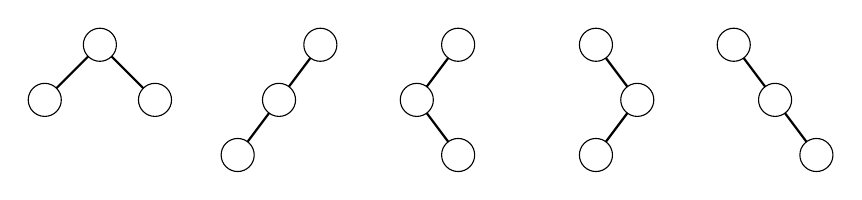
\begin{tikzpicture}[scale=0.7]
\path[draw,thick,-] (0,0) -- (-1,-1);
\path[draw,thick,-] (0,0) -- (1,-1);
\draw[fill=white] (0,0) circle (0.3);
\draw[fill=white] (-1,-1) circle (0.3);
\draw[fill=white] (1,-1) circle (0.3);

\path[draw,thick,-] (4,0) -- (4-0.75,-1) -- (4-1.5,-2);
\draw[fill=white] (4,0) circle (0.3);
\draw[fill=white] (4-0.75,-1) circle (0.3);
\draw[fill=white] (4-1.5,-2) circle (0.3);

\path[draw,thick,-] (6.5,0) -- (6.5-0.75,-1) -- (6.5-0,-2);
\draw[fill=white] (6.5,0) circle (0.3);
\draw[fill=white] (6.5-0.75,-1) circle (0.3);
\draw[fill=white] (6.5-0,-2) circle (0.3);

\path[draw,thick,-] (9,0) -- (9+0.75,-1) -- (9-0,-2);
\draw[fill=white] (9,0) circle (0.3);
\draw[fill=white] (9+0.75,-1) circle (0.3);
\draw[fill=white] (9-0,-2) circle (0.3);

\path[draw,thick,-] (11.5,0) -- (11.5+0.75,-1) -- (11.5+1.5,-2);
\draw[fill=white] (11.5,0) circle (0.3);
\draw[fill=white] (11.5+0.75,-1) circle (0.3);
\draw[fill=white] (11.5+1.5,-2) circle (0.3);
\end{tikzpicture}
\end{center}
and the rooted trees are
\begin{center}
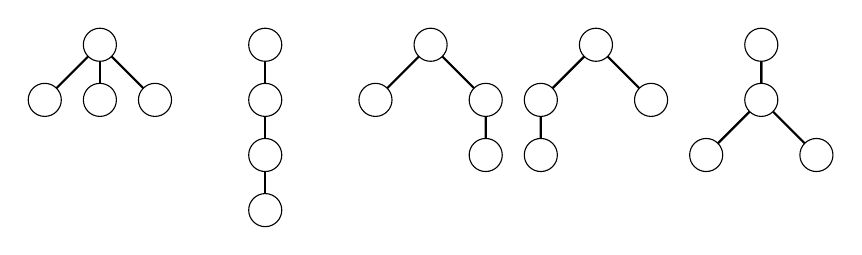
\begin{tikzpicture}[scale=0.7]
\path[draw,thick,-] (0,0) -- (-1,-1);
\path[draw,thick,-] (0,0) -- (0,-1);
\path[draw,thick,-] (0,0) -- (1,-1);
\draw[fill=white] (0,0) circle (0.3);
\draw[fill=white] (-1,-1) circle (0.3);
\draw[fill=white] (0,-1) circle (0.3);
\draw[fill=white] (1,-1) circle (0.3);

\path[draw,thick,-] (3,0) -- (3,-1) -- (3,-2) -- (3,-3);
\draw[fill=white] (3,0) circle (0.3);
\draw[fill=white] (3,-1) circle (0.3);
\draw[fill=white] (3,-2) circle (0.3);
\draw[fill=white] (3,-3) circle (0.3);

\path[draw,thick,-] (6+0,0) -- (6-1,-1);
\path[draw,thick,-] (6+0,0) -- (6+1,-1) -- (6+1,-2);
\draw[fill=white] (6+0,0) circle (0.3);
\draw[fill=white] (6-1,-1) circle (0.3);
\draw[fill=white] (6+1,-1) circle (0.3);
\draw[fill=white] (6+1,-2) circle (0.3);

\path[draw,thick,-] (9+0,0) -- (9+1,-1);
\path[draw,thick,-] (9+0,0) -- (9-1,-1) -- (9-1,-2);
\draw[fill=white] (9+0,0) circle (0.3);
\draw[fill=white] (9+1,-1) circle (0.3);
\draw[fill=white] (9-1,-1) circle (0.3);
\draw[fill=white] (9-1,-2) circle (0.3);

\path[draw,thick,-] (12+0,0) -- (12+0,-1) -- (12-1,-2);
\path[draw,thick,-] (12+0,0) -- (12+0,-1) -- (12+1,-2);
\draw[fill=white] (12+0,0) circle (0.3);
\draw[fill=white] (12+0,-1) circle (0.3);
\draw[fill=white] (12-1,-2) circle (0.3);
\draw[fill=white] (12+1,-2) circle (0.3);

\end{tikzpicture}
\end{center}

\section{Inclusion-exclusion}

\index{inclusion-exclusion}

\key{Inclusion-exclusion} is a technique
that can be used for counting the size
of a union of sets when the sizes of
the intersections are known, and vice versa.
A simple example of the technique is the formula
\[ |A \cup B| = |A| + |B| - |A \cap B|,\]
where $A$ and $B$ are sets and $|X|$
denotes the size of $X$.
The formula can be illustrated as follows:

\begin{center}
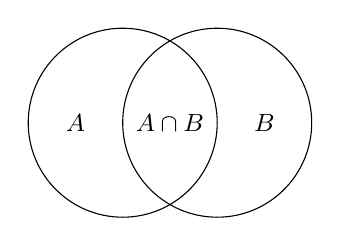
\begin{tikzpicture}[scale=0.8]

\draw (0,0) circle (1.5);
\draw (1.5,0) circle (1.5);

\node at (-0.75,0) {\small $A$};
\node at (2.25,0) {\small $B$};
\node at (0.75,0) {\small $A \cap B$};

\end{tikzpicture}
\end{center}

Our goal is to calculate
the size of the union $A \cup B$
that corresponds to the area of the region
that belongs to at least one circle.
The picture shows that we can calculate
the area of $A \cup B$ by first summing the
areas of $A$ and $B$ and then subtracting
the area of $A \cap B$.

The same idea can be applied when the number
of sets is larger.
When there are three sets, the inclusion-exclusion formula is
\[ |A \cup B \cup C| = |A| + |B| + |C| - |A \cap B|  - |A \cap C|  - |B \cap C| + |A \cap B \cap C| \]
and the corresponding picture is

\begin{center}
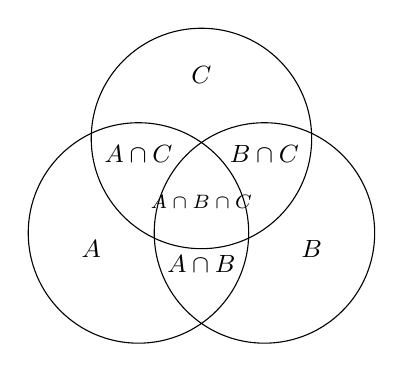
\begin{tikzpicture}[scale=0.8]

\draw (0,0) circle (1.75);
\draw (2,0) circle (1.75);
\draw (1,1.5) circle (1.75);

\node at (-0.75,-0.25) {\small $A$};
\node at (2.75,-0.25) {\small $B$};
\node at (1,2.5) {\small $C$};
\node at (1,-0.5) {\small $A \cap B$};
\node at (0,1.25) {\small $A \cap C$};
\node at (2,1.25) {\small $B \cap C$};
\node at (1,0.5) {\scriptsize $A \cap B \cap C$};

\end{tikzpicture}
\end{center}

In the general case, the size of the 
union $X_1 \cup X_2 \cup \cdots \cup X_n$
can be calculated by going through all possible
intersections that contain some of the sets $X_1,X_2,\ldots,X_n$.
If the intersection contains an odd number of sets,
its size is added to the answer,
and otherwise its size is subtracted from the answer.

Note that there are similar formulas
for calculating
the size of an intersection from the sizes of
unions. For example,
\[ |A \cap B| = |A| + |B| - |A \cup B|\]
and
\[ |A \cap B \cap C| = |A| + |B| + |C| - |A \cup B|  - |A \cup C|  - |B \cup C| + |A \cup B \cup C| .\]

\subsubsection{Derangements}

\index{derangement}

As an example, let us count the number of \key{derangements}
of elements $\{1,2,\ldots,n\}$, i.e., permutations
where no element remains in its original place.
For example, when $n=3$, there are
two derangements: $(2,3,1)$ and $(3,1,2)$.

One approach for solving the problem is to use
inclusion-exclusion.
Let $X_k$ be the set of permutations
that contain the element $k$ at position $k$.
For example, when $n=3$, the sets are as follows:
\[
\begin{array}{lcl}
X_1 & = & \{(1,2,3),(1,3,2)\} \\
X_2 & = & \{(1,2,3),(3,2,1)\} \\
X_3 & = & \{(1,2,3),(2,1,3)\} \\
\end{array}
\]
Using these sets, the number of derangements equals
\[ n! - |X_1 \cup X_2 \cup \cdots \cup X_n|, \]
so it suffices to calculate the size of the union.
Using inclusion-exclusion, this reduces to
calculating sizes of intersections which can be
done efficiently.
For example, when $n=3$, the size of
$|X_1 \cup X_2 \cup X_3|$ is
\[
\begin{array}{lcl}
 & & |X_1| + |X_2| + |X_3| - |X_1 \cap X_2|  - |X_1 \cap X_3|  - |X_2 \cap X_3| + |X_1 \cap X_2 \cap X_3| \\
 & = & 2+2+2-1-1-1+1 \\
 & = & 4, \\
\end{array}
\]
so the number of solutions is $3!-4=2$.

It turns out that the problem can also be solved
without using inclusion-exclusion.
Let $f(n)$ denote the number of derangements
for $\{1,2,\ldots,n\}$. We can use the following
recursive formula:

\begin{equation*}
    f(n) = \begin{cases}
               0               & n = 1\\
               1               & n = 2\\
               (n-1)(f(n-2) + f(n-1)) & n>2 \\
           \end{cases}
\end{equation*}

The formula can be derived by considering
the possibilities how the element 1 changes
in the derangement.
There are $n-1$ ways to choose an element $x$
that replaces the element 1.
In each such choice, there are two options:

\textit{Option 1:} We also replace the element $x$
with the element 1.
After this, the remaining task is to construct
a derangement of $n-2$ elements.

\textit{Option 2:} We replace the element $x$
with some other element than 1.
Now we have to construct a derangement
of $n-1$ element, because we cannot replace
the element $x$ with the element $1$, and all other
elements must be changed.

\section{Burnside's lemma}

\index{Burnside's lemma}

\key{Burnside's lemma}
%\footnote{Actually, Burnside did not discover this lemma; he only mentioned it in his book \cite{bur97}.}
can be used to count
the number of combinations so that
only one representative is counted
for each group of symmetric combinations.
Burnside's lemma states that the number of
combinations is
\[\sum_{k=1}^n \frac{c(k)}{n},\]
where there are $n$ ways to change the
position of a combination,
and there are $c(k)$ combinations that
remain unchanged when the $k$th way is applied.

As an example, let us calculate the number of
necklaces of $n$ pearls,
where each pearl has $m$ possible colors.
Two necklaces are symmetric if they are
similar after rotating them.
For example, the necklace
\begin{center}
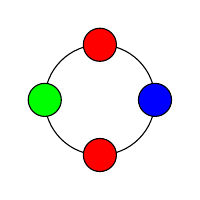
\begin{tikzpicture}[scale=0.7]
\draw[fill=white] (0,0) circle (1);
\draw[fill=red] (0,1) circle (0.3);
\draw[fill=blue] (1,0) circle (0.3);
\draw[fill=red] (0,-1) circle (0.3);
\draw[fill=green] (-1,0) circle (0.3);
\end{tikzpicture}
\end{center}
has the following symmetric necklaces:
\begin{center}
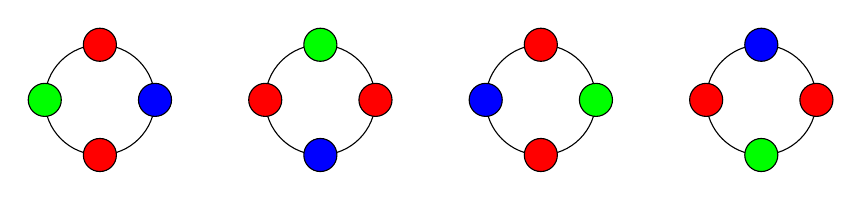
\begin{tikzpicture}[scale=0.7]
\draw[fill=white] (0,0) circle (1);
\draw[fill=red] (0,1) circle (0.3);
\draw[fill=blue] (1,0) circle (0.3);
\draw[fill=red] (0,-1) circle (0.3);
\draw[fill=green] (-1,0) circle (0.3);

\draw[fill=white] (4,0) circle (1);
\draw[fill=green] (4+0,1) circle (0.3);
\draw[fill=red] (4+1,0) circle (0.3);
\draw[fill=blue] (4+0,-1) circle (0.3);
\draw[fill=red] (4+-1,0) circle (0.3);

\draw[fill=white] (8,0) circle (1);
\draw[fill=red] (8+0,1) circle (0.3);
\draw[fill=green] (8+1,0) circle (0.3);
\draw[fill=red] (8+0,-1) circle (0.3);
\draw[fill=blue] (8+-1,0) circle (0.3);

\draw[fill=white] (12,0) circle (1);
\draw[fill=blue] (12+0,1) circle (0.3);
\draw[fill=red] (12+1,0) circle (0.3);
\draw[fill=green] (12+0,-1) circle (0.3);
\draw[fill=red] (12+-1,0) circle (0.3);
\end{tikzpicture}
\end{center}
There are $n$ ways to change the position
of a necklace,
because we can rotate it
$0,1,\ldots,n-1$ steps clockwise.
If the number of steps is 0,
all $m^n$ necklaces remain the same,
and if the number of steps is 1,
only the $m$ necklaces where each
pearl has the same color remain the same.

More generally, when the number of steps is $k$,
a total of
\[m^{\textrm{gcd}(k,n)}\]
necklaces remain the same,
where $\textrm{gcd}(k,n)$ is the greatest common
divisor of $k$ and $n$.
The reason for this is that blocks
of pearls of size $\textrm{gcd}(k,n)$
will replace each other.
Thus, according to Burnside's lemma,
the number of necklaces is
\[\sum_{i=0}^{n-1} \frac{m^{\textrm{gcd}(i,n)}}{n}. \]
For example, the number of necklaces of length 4
with 3 colors is
\[\frac{3^4+3+3^2+3}{4} = 24. \]

\section{Cayley's formula}

\index{Cayley's formula}

\key{Cayley's formula}
% \footnote{While the formula is named after A. Cayley,
% who studied it in 1889, it was discovered earlier by C. W. Borchardt in 1860.}
states that
there are $n^{n-2}$ labeled trees
that contain $n$ nodes.
The nodes are labeled $1,2,\ldots,n$,
and two trees are different
if either their structure or
labeling is different.

\begin{samepage}
For example, when $n=4$, the number of labeled
trees is $4^{4-2}=16$:

\begin{center}
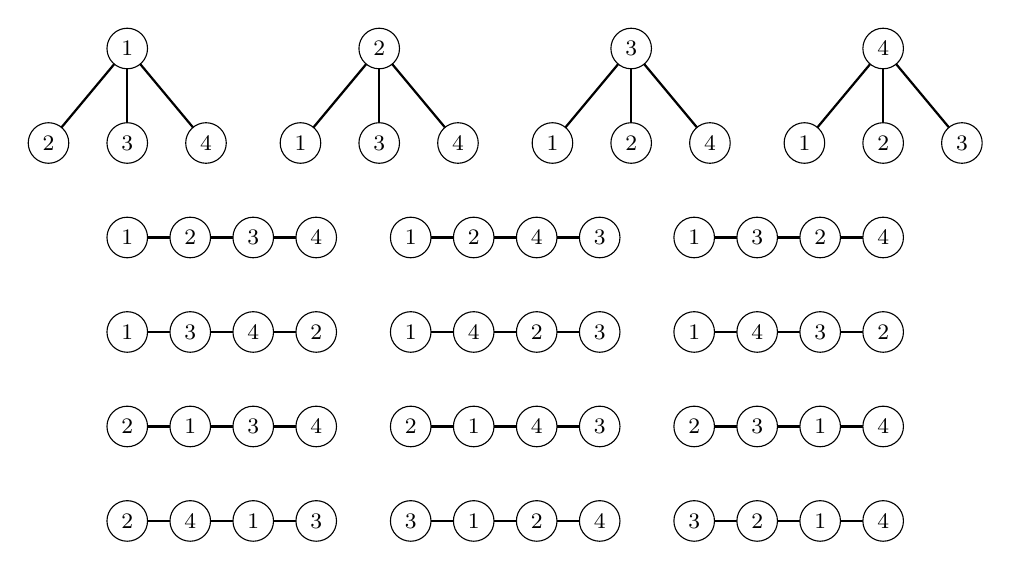
\begin{tikzpicture}[scale=0.8]
\footnotesize

\newcommand\puua[6]{
\path[draw,thick,-] (#1,#2) -- (#1-1.25,#2-1.5);
\path[draw,thick,-] (#1,#2) -- (#1,#2-1.5);
\path[draw,thick,-] (#1,#2) -- (#1+1.25,#2-1.5);
\node[draw, circle, fill=white] at (#1,#2) {#3};
\node[draw, circle, fill=white] at (#1-1.25,#2-1.5) {#4};
\node[draw, circle, fill=white] at (#1,#2-1.5) {#5};
\node[draw, circle, fill=white] at (#1+1.25,#2-1.5) {#6};
}
\newcommand\puub[6]{
\path[draw,thick,-] (#1,#2) -- (#1+1,#2);
\path[draw,thick,-] (#1+1,#2) -- (#1+2,#2);
\path[draw,thick,-] (#1+2,#2) -- (#1+3,#2);
\node[draw, circle, fill=white] at (#1,#2) {#3};
\node[draw, circle, fill=white] at (#1+1,#2) {#4};
\node[draw, circle, fill=white] at (#1+2,#2) {#5};
\node[draw, circle, fill=white] at (#1+3,#2) {#6};
}

\puua{0}{0}{1}{2}{3}{4}
\puua{4}{0}{2}{1}{3}{4}
\puua{8}{0}{3}{1}{2}{4}
\puua{12}{0}{4}{1}{2}{3}

\puub{0}{-3}{1}{2}{3}{4}
\puub{4.5}{-3}{1}{2}{4}{3}
\puub{9}{-3}{1}{3}{2}{4}
\puub{0}{-4.5}{1}{3}{4}{2}
\puub{4.5}{-4.5}{1}{4}{2}{3}
\puub{9}{-4.5}{1}{4}{3}{2}
\puub{0}{-6}{2}{1}{3}{4}
\puub{4.5}{-6}{2}{1}{4}{3}
\puub{9}{-6}{2}{3}{1}{4}
\puub{0}{-7.5}{2}{4}{1}{3}
\puub{4.5}{-7.5}{3}{1}{2}{4}
\puub{9}{-7.5}{3}{2}{1}{4}
\end{tikzpicture}
\end{center}
\end{samepage}

Next we will see how Cayley's formula can
be derived using Prüfer codes.

\subsubsection{Prüfer code}

\index{Prüfer code}

A \key{Prüfer code}
%\footnote{In 1918, H. Prüfer proved Cayley's theorem using Prüfer codes \cite{pru18}.}
is a sequence of
$n-2$ numbers that describes a labeled tree.
The code is constructed by following a process
that removes $n-2$ leaves from the tree.
At each step, the leaf with the smallest label is removed,
and the label of its only neighbor is added to the code.

For example, let us calculate the Prüfer code
of the following graph:
\begin{center}
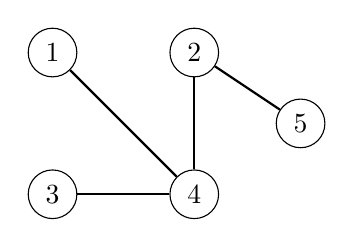
\begin{tikzpicture}[scale=0.9]
\node[draw, circle] (1) at (2,3) {$1$};
\node[draw, circle] (2) at (4,3) {$2$};
\node[draw, circle] (3) at (2,1) {$3$};
\node[draw, circle] (4) at (4,1) {$4$};
\node[draw, circle] (5) at (5.5,2) {$5$};

\path[draw,thick,-] (1) -- (4);
\path[draw,thick,-] (3) -- (4);
\path[draw,thick,-] (2) -- (4);
\path[draw,thick,-] (2) -- (5);
\end{tikzpicture}
\end{center}

First we remove node 1 and add node 4 to the code:
\begin{center}
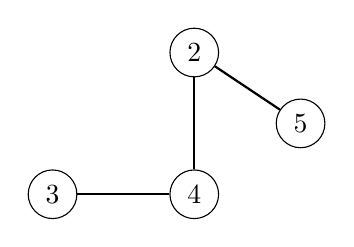
\begin{tikzpicture}[scale=0.9]
%\node[draw, circle] (1) at (2,3) {$1$};
\node[draw, circle] (2) at (4,3) {$2$};
\node[draw, circle] (3) at (2,1) {$3$};
\node[draw, circle] (4) at (4,1) {$4$};
\node[draw, circle] (5) at (5.5,2) {$5$};

%\path[draw,thick,-] (1) -- (4);
\path[draw,thick,-] (3) -- (4);
\path[draw,thick,-] (2) -- (4);
\path[draw,thick,-] (2) -- (5);
\end{tikzpicture}
\end{center}

Then we remove node 3 and add node 4 to the code:
\begin{center}
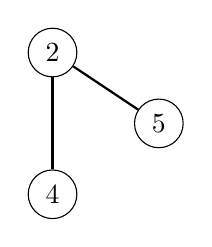
\begin{tikzpicture}[scale=0.9]
%\node[draw, circle] (1) at (2,3) {$1$};
\node[draw, circle] (2) at (4,3) {$2$};
%\node[draw, circle] (3) at (2,1) {$3$};
\node[draw, circle] (4) at (4,1) {$4$};
\node[draw, circle] (5) at (5.5,2) {$5$};

%\path[draw,thick,-] (1) -- (4);
%\path[draw,thick,-] (3) -- (4);
\path[draw,thick,-] (2) -- (4);
\path[draw,thick,-] (2) -- (5);
\end{tikzpicture}
\end{center}

Finally we remove node 4 and add node 2 to the code:
\begin{center}
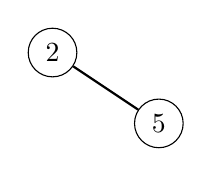
\begin{tikzpicture}[scale=0.9]
%\node[draw, circle] (1) at (2,3) {$1$};
\node[draw, circle] (2) at (4,3) {$2$};
%\node[draw, circle] (3) at (2,1) {$3$};
%\node[draw, circle] (4) at (4,1) {$4$};
\node[draw, circle] (5) at (5.5,2) {$5$};

%\path[draw,thick,-] (1) -- (4);
%\path[draw,thick,-] (3) -- (4);
%\path[draw,thick,-] (2) -- (4);
\path[draw,thick,-] (2) -- (5);
\end{tikzpicture}
\end{center}

Thus, the Prüfer code of the graph is $[4,4,2]$.

We can construct a Prüfer code for any tree,
and more importantly,
the original tree can be reconstructed
from a Prüfer code.
Hence, the number of labeled trees
of $n$ nodes equals
$n^{n-2}$, the number of Prüfer codes
of size $n$.
